%\documentclass{article}
%\usepackage{beamerarticle}
\documentclass[serif,ignorenonframetext]{beamer}

% Macros for MATH 110 course dates

\newcommand{\commonTheme}{metropolis}
\newcommand{\commonColorTheme}{metropolis}

\newcommand{\commonAuthor}{Edward Doolittle}
\newcommand{\commonInstitute}{Department of Indigenous Knowledge and
  Science \\ First Nations University of Canada}
\newcommand{\commonCourse}{MATH 110 Calculus I}
\newcommand{\commonTerm}{202510}
\newcommand{\commonDate}{January 6, 2025}

% Review Material

% Lab 0
\newcommand{\commonEventNegativeOne}{LabNegativeOne}
\newcommand{\commonDateLabNegativeOne}{Monday, January 6, 2025}
\newcommand{\commonTitleLabNegativeOne}{MATH 110 Lab 0}
\newcommand{\commonSubtitleLabNegativeOne}{No Lab; Course Opens}

% Section 001
\newcommand{\commonEventZeroZeroOne}{ZeroZeroOne}
\newcommand{\commonDateZeroZeroOne}{Tuesday, January 7, 2025}
\newcommand{\commonTitleZeroZeroOne}{MATH 110 Review 0.1}
\newcommand{\commonSubtitleZeroZeroOne}{Review of Algebra}
\newcommand{\commonPSTitleZeroZeroOne}{MATH 110 Review Problem Set 0.1}

% Section 00A
\newcommand{\commonEventZeroZeroA}{ZeroZeroA}
\newcommand{\commonDateZeroZeroA}{Tuesday, January 7, 2025}
\newcommand{\commonTitleZeroZeroA}{MATH 110 Review 0.A}
\newcommand{\commonSubtitleZeroZeroA}{Review of Inequalities and
  Absolute Values}
\newcommand{\commonPSTitleZeroZeroA}{MATH 110 Review Problem Set 0.A}

% Section 00B
\newcommand{\commonEventZeroZeroB}{ZeroZeroB}
\newcommand{\commonDateZeroZeroB}{Tuesday, January 7, 2025}
\newcommand{\commonTitleZeroZeroB}{MATH 110 Review 0.B}
\newcommand{\commonSubtitleZeroZeroB}{Review of Coordinate Geometry
  and Lines}
\newcommand{\commonPSTitleZeroZeroB}{MATH 110 Review Problem Set 0.B}

% Section 00C
\newcommand{\commonEventZeroZeroC}{ZeroZeroC}
\newcommand{\commonDateZeroZeroC}{Thursday, January 9, 2025}
\newcommand{\commonTitleZeroZeroC}{MATH 110 Review 0.C}
\newcommand{\commonSubtitleZeroZeroC}{Review of Graphs of Second
  Degree Equations}
\newcommand{\commonPSTitleZeroZeroC}{MATH 110 Review Problem Set 0.C}

% Section 00D
\newcommand{\commonEventZeroZeroD}{ZeroZeroD}
\newcommand{\commonDateZeroZeroD}{Thursday, January 9, 2025}
\newcommand{\commonTitleZeroZeroD}{MATH 110 Review 0.D}
\newcommand{\commonSubtitleZeroZeroD}{Review of Trigonometry}
\newcommand{\commonPSTitleZeroZeroD}{MATH 110 Review Problem Set 0.D}

% Section 011
\newcommand{\commonEventZeroOneOne}{ZeroOneOne}
\newcommand{\commonDateZeroOneOne}{Thursday, January 9, 2025}
\newcommand{\commonTitleZeroOneOne}{MATH 110 Review 1.1}
\newcommand{\commonSubtitleZeroOneOne}{Review of Functions}
\newcommand{\commonPSTitleZeroOneOne}{MATH 110 Review Problem Set 1.1}


% Main Course

% Lab 1
\newcommand{\commonEventZero}{LabZero}
\newcommand{\commonDateLabZero}{Monday, January 13, 2025}
\newcommand{\commonTitleLabZero}{MATH 110 Lab 1}
\newcommand{\commonSubtitleLabZero}{Quiz 0: STACK, Onboarding}

% Section 1.4
\newcommand{\commonEventOne}{ZeroOneFour}
\newcommand{\commonDateZeroOneFour}{Tuesday, January 14, 2025}
\newcommand{\commonTitleZeroOneFour}{MATH 110 Lecture 1.4}
\newcommand{\commonSubtitleZeroOneFour}{The Tangent and Velocity Problems}
\newcommand{\commonPSTitleZeroOneFour}{MATH 110 Problem Set 1.4}

% Section 1.5
\newcommand{\commonEventTwo}{ZeroOneFive}
\newcommand{\commonDateZeroOneFive}{Thursday, January 16, 2025}
\newcommand{\commonTitleZeroOneFive}{MATH 110 Lecture 1.5}
\newcommand{\commonSubtitleZeroOneFive}{The Limit of a Function}
\newcommand{\commonPSTitleZeroOneFive}{MATH 110 Problem Set 1.5}

% Lab 2
\newcommand{\commonEventThree}{LabOne}
\newcommand{\commonDateLabOne}{Monday, January 20, 2025}
\newcommand{\commonTitleLabOne}{MATH 110 Lab 2}
\newcommand{\commonSubtitleLabOne}{Quiz 1: Review}

% Section 1.6
\newcommand{\commonEventFour}{ZeroOneSix}
\newcommand{\commonDateZeroOneSix}{Tuesday, January 21, 2025}
\newcommand{\commonTitleZeroOneSix}{MATH 110 Lecture 1.6}
\newcommand{\commonSubtitleZeroOneSix}{Calculating Limits Using the Limit Laws}
\newcommand{\commonPSTitleZeroOneSix}{MATH 110 Problem Set 1.6}

% Section 1.7
\newcommand{\commonEventFive}{ZeroOneSeven}
\newcommand{\commonDateZeroOneSeven}{(Not covered)}
\newcommand{\commonTitleZeroOneSeven}{MATH 110 Lecture 1.7}
\newcommand{\commonSubtitleZeroOneSeven}{The Precise Definition of a Limit}
\newcommand{\commonPSTitleZeroOneSeven}{MATH 110 Problem Set 1.7}

% Section 1.8
\newcommand{\commonEventSix}{ZeroOneEight}
\newcommand{\commonDateZeroOneEight}{Thursday, January 23, 2025}
\newcommand{\commonTitleZeroOneEight}{MATH 110 Lecture 1.8}
\newcommand{\commonSubtitleZeroOneEight}{Continuity}
\newcommand{\commonPSTitleZeroOneEight}{MATH 110 Problem Set 1.8}

% Lab 3
\newcommand{\commonEventSeven}{LabTwo}
\newcommand{\commonDateLabTwo}{Monday, January 27, 2025}
\newcommand{\commonTitleLabTwo}{MATH 110 Lab 3}
\newcommand{\commonSubtitleLabTwo}{Quiz 2: Sections 1.4, 1.5}

% Section 2.1
\newcommand{\commonEventEight}{ZeroTwoOne}
\newcommand{\commonDateZeroTwoOne}{Tuesday, January 28, 2025}
\newcommand{\commonTitleZeroTwoOne}{MATH 110 Lecture 2.1}
\newcommand{\commonSubtitleZeroTwoOne}{Derivatives and Rates of Change}
\newcommand{\commonPSTitleZeroTwoOne}{MATH 110 Problem Set 2.1}

% Section 2.2
\newcommand{\commonEventNine}{ZeroTwoTwo}
\newcommand{\commonDateZeroTwoTwo}{Thursday, January 30, 2025}
\newcommand{\commonTitleZeroTwoTwo}{MATH 110 Lecture 2.2}
\newcommand{\commonSubtitleZeroTwoTwo}{The Derivative as a Function}
\newcommand{\commonPSTitleZeroTwoTwo}{MATH 110 Problem Set 2.2}

% Lab 4
\newcommand{\commonEventTen}{LabThree}
\newcommand{\commonDateMTOne}{Monday, February 3, 2025} 
\newcommand{\commonDateLabThree}{Monday, February 3, 2025}
\newcommand{\commonTitleLabThree}{MATH 110 Lab 4}
\newcommand{\commonSubtitleLabThree}{Midterm: Review, Chapter 1}

% Section 2.3
\newcommand{\commonEventEleven}{ZeroTwoThree}
\newcommand{\commonDateZeroTwoThree}{Tuesday, February 4, 2025}
\newcommand{\commonTitleZeroTwoThree}{MATH 110 Lecture 2.3}
\newcommand{\commonSubtitleZeroTwoThree}{Differentiation Formulas}
\newcommand{\commonPSTitleZeroTwoThree}{MATH 110 Problem Set 2.3}

% Section 2.4
\newcommand{\commonEventTwelve}{ZeroTwoFour}
\newcommand{\commonDateZeroTwoFour}{Thursday, February 6, 2025}
\newcommand{\commonTitleZeroTwoFour}{MATH 110 Lecture 2.4}
\newcommand{\commonSubtitleZeroTwoFour}{Derivatives of Trigonometric Functions}
\newcommand{\commonPSTitleZeroTwoFour}{MATH 110 Problem Set 2.4}

% Lab 5
\newcommand{\commonEventThirteen}{LabFour}
\newcommand{\commonDateLabFour}{Monday, February 10, 2025}
\newcommand{\commonTitleLabFour}{MATH 110 Lab 5}
\newcommand{\commonSubtitleLabFour}{Quiz 3: Sections 2.1, 2.2}

% Section 2.5
\newcommand{\commonEventFourteen}{ZeroTwoFive}
\newcommand{\commonDateZeroTwoFive}{Tuesday, February 11, 2025}
\newcommand{\commonTitleZeroTwoFive}{MATH 110 Lecture 2.5}
\newcommand{\commonSubtitleZeroTwoFive}{The Chain Rule}
\newcommand{\commonPSTitleZeroTwoFive}{MATH 110 Problem Set 2.5}

% Section 2.6
\newcommand{\commonEventFifteen}{ZeroTwoSix}
\newcommand{\commonDateZeroTwoSix}{Thursday, February 13, 2025}
\newcommand{\commonTitleZeroTwoSix}{MATH 110 Lecture 2.6}
\newcommand{\commonSubtitleZeroTwoSix}{Implicit Differentiation}
\newcommand{\commonPSTitleZeroTwoSix}{MATH 110 Problem Set 2.6}

% Lab 6
\newcommand{\commonEventSixteen}{LabFive}
\newcommand{\commonDateLabFive}{Monday, February 24, 2025}
\newcommand{\commonTitleLabFive}{MATH 110 Lab 6}
\newcommand{\commonSubtitleLabFive}{Quiz 4: Sections 2.3, 2.4}

% Section 2.7
\newcommand{\commonEventSeventeen}{ZeroTwoSeven}
\newcommand{\commonDateZeroTwoSeven}{Tuesday, February 25, 2025}
\newcommand{\commonTitleZeroTwoSeven}{MATH 110 Lecture 2.7}
\newcommand{\commonSubtitleZeroTwoSeven}{Rates of Change in the
  Natural and Social Sciences}
\newcommand{\commonPSTitleZeroTwoSeven}{MATH 110 Problem Set 2.7}

% Section 2.8
\newcommand{\commonEventEighteen}{ZeroTwoEight}
\newcommand{\commonDateZeroTwoEight}{Thursday, February 27, 2025}
\newcommand{\commonTitleZeroTwoEight}{MATH 110 Lecture 2.8}
\newcommand{\commonSubtitleZeroTwoEight}{Related Rates}
\newcommand{\commonPSTitleZeroTwoEight}{MATH 110 Problem Set 2.8}

% Lab 7
\newcommand{\commonEventNineteen}{LabSix}
\newcommand{\commonDateLabSix}{Monday, March 3, 2025}
\newcommand{\commonTitleLabSix}{MATH 110 Lab 7}
\newcommand{\commonSubtitleLabSix}{Quiz 5: Sections 2.5, 2.6}

% Section 3.1
\newcommand{\commonEventTwenty}{ZeroThreeOne}
\newcommand{\commonDateZeroThreeOne}{Tuesday, March 4, 2025}
\newcommand{\commonTitleZeroThreeOne}{MATH 110 Lecture 3.1}
\newcommand{\commonSubtitleZeroThreeOne}{Maximum and Minimum Values}
\newcommand{\commonPSTitleZeroThreeOne}{MATH 11 Problem Set 3.1}

% Section 3.2
\newcommand{\commonEventTwentyOne}{ZeroThreeTwo}
\newcommand{\commonDateZeroThreeTwo}{Thursday, March 6, 2025}
\newcommand{\commonTitleZeroThreeTwo}{MATH 110 Lecture 3.2}
\newcommand{\commonSubtitleZeroThreeTwo}{The Mean Value Theorem}
\newcommand{\commonPSTitleZeroThreeTwo}{MATH 110 Problem Set 3.2}

% Lab 8
\newcommand{\commonEventTwentyTwo}{LabSeven}
\newcommand{\commonDateMTTwo}{Monday, March 10, 2025}
\newcommand{\commonDateLabSeven}{Monday, March 10, 2025}
\newcommand{\commonTitleLabSeven}{MATH 110 Lab 8}
\newcommand{\commonSubtitleLabSeven}{Midterm: Chapter 2}

% Section 3.3
\newcommand{\commonEventTwentyThree}{ZeroThreeThree}
\newcommand{\commonDateZeroThreeThree}{Tuesday, March 11, 2025}
\newcommand{\commonTitleZeroThreeThree}{MATH 110 Lecture 3.3}
\newcommand{\commonSubtitleZeroThreeThree}{How Derivatives Affect the
  Shape of a Graph}
\newcommand{\commonPSTitleZeroThreeThree}{MATH 110 Problem Set 3.3}

% Section 3.4
\newcommand{\commonEventTwentyFour}{ZeroThreeFour}
\newcommand{\commonDateZeroThreeFour}{Thursday, March 13, 2025}
\newcommand{\commonTitleZeroThreeFour}{MATH 110 Lecture 3.4}
\newcommand{\commonSubtitleZeroThreeFour}{Limits at Infinity;
  Horizontal Asymptotes}
\newcommand{\commonPSTitleZeroThreeFour}{MATH 110 Problem Set 3.4}

% Lab 9
\newcommand{\commonEventTwentyFive}{LabEight}
\newcommand{\commonDateLabEight}{Monday, March 17, 2025}
\newcommand{\commonTitleLabEight}{MATH 110 Lab 9}
\newcommand{\commonSubtitleLabEight}{Quiz 6: Sections 3.1, 3.2}

% Section 3.5
\newcommand{\commonEventTwentySix}{ZeroThreeFive}
\newcommand{\commonDateZeroThreeFive}{Tuesday, March 18, 2025}
\newcommand{\commonTitleZeroThreeFive}{MATH 110 Lecture 3.5}
\newcommand{\commonSubtitleZeroThreeFive}{Summary of Curve Sketching}
\newcommand{\commonPSTitleZeroThreeFive}{MATH 110 Problem Set 3.5}

% Section 3.7
\newcommand{\commonEventTwentySeven}{ZeroThreeSeven}
\newcommand{\commonDateZeroThreeSeven}{Thursday, March 20, 2025}
\newcommand{\commonTitleZeroThreeSeven}{MATH 110 Lecture 3.7}
\newcommand{\commonSubtitleZeroThreeSeven}{Optimization Problems}
\newcommand{\commonPSTitleZeroThreeSeven}{MATH 110 Problem Set 3.7}

% Lab 10
\newcommand{\commonEventTwentyEight}{LabNine}
\newcommand{\commonDateLabNine}{Monday, March 24, 2025}
\newcommand{\commonTitleLabNine}{MATH 110 Lab 10}
\newcommand{\commonSubtitleLabNine}{Quiz 7: Sections 3.3, 3.4}

% Section 4.1
\newcommand{\commonEventTwentyNine}{ZeroFourOne}
\newcommand{\commonDateZeroFourOne}{Tuesday, March 25, 2025}
\newcommand{\commonTitleZeroFourOne}{MATH 110 Lecture 4.1}
\newcommand{\commonSubtitleZeroFourOne}{Areas and Distances}
\newcommand{\commonPSTitleZeroFourOne}{MATH 110 Problem Set 4.1}

% Section 4.2
\newcommand{\commonEventThirty}{ZeroFourTwo}
\newcommand{\commonDateZeroFourTwo}{Thursday, March 27, 2025}
\newcommand{\commonTitleZeroFourTwo}{MATH 110 Lecture 4.2}
\newcommand{\commonSubtitleZeroFourTwo}{The Definite Integral}
\newcommand{\commonPSTitleZeroFourTwo}{MATH 110 Problem Set 4.2}

% Lab 11
\newcommand{\commonEventThirtyOne}{LabTen}
\newcommand{\commonDateLabTen}{Monday, March 31, 2025}
\newcommand{\commonTitleLabTen}{MATH 110 Lab 11}
\newcommand{\commonSubtitleLabTen}{Quiz 8: Sections 3.5, 3.7}

% Section 4.3
\newcommand{\commonEventThirtyTwo}{ZeroFourThree}
\newcommand{\commonDateZeroFourThree}{Tuesday, April 1, 2025}
\newcommand{\commonTitleZeroFourThree}{MATH 110 Lecture 4.3}
\newcommand{\commonSubtitleZeroFourThree}{The Fundamental Theorem of Calculus}
\newcommand{\commonPSTitleZeroFourThree}{MATH 110 Problem Set 4.3}

% Section 4.4
\newcommand{\commonEventThirtyThree}{ZeroFourFour}
\newcommand{\commonDateZeroFourFour}{Thursday, April 3, 2025}
\newcommand{\commonTitleZeroFourFour}{MATH 110 Lecture 4.4}
\newcommand{\commonSubtitleZeroFourFour}{Indefinite Integrals and the
  Net Change Theorem}
\newcommand{\commonPSTitleZeroFourFour}{MATH 110 Problem Set 4.4}

% Lab 12
\newcommand{\commonEventThirtyFour}{LabEleven}
\newcommand{\commonDateLabEleven}{Monday, April 7, 2025}
\newcommand{\commonTitleLabEleven}{MATH 110 Lab 12}
\newcommand{\commonSubtitleLabEleven}{Quiz 9: Sections 4.1, 4.2}

% Section 4.5
\newcommand{\commonEventThirtyFive}{ZeroFourFive}
\newcommand{\commonDateZeroFourFive}{Tuesday, April 8, 2025}
\newcommand{\commonTitleZeroFourFive}{MATH 110 Lecture 4.5}
\newcommand{\commonSubtitleZeroFourFive}{The Substitution Rule}
\newcommand{\commonPSTitleZeroFourFive}{MATH 110 Problem Set 4.5}

% Section 5.1
\newcommand{\commonEventThirtySix}{ZeroFiveOne}
\newcommand{\commonDateZeroFiveOne}{Thursday, April 10, 2025}
\newcommand{\commonTitleZeroFiveOne}{MATH 110 Lecture 5.1}
\newcommand{\commonSubtitleZeroFiveOne}{Areas Between Curves}
\newcommand{\commonPSTitleZeroFiveOne}{MATH 110 Problem Set 5.1}

% Lab 13
\newcommand{\commonEventThirtySeven}{LabTwelve}
\newcommand{\commonDateLabTwelve}{Monday, April 14, 2025}
\newcommand{\commonTitleLabTwelve}{MATH 110 Review Lab}
\newcommand{\commonSubtitleLabTwelve}{Bonus Quiz 10: Sections 4.3, 4.4}

% Final Class
\newcommand{\commonEventThirtyEight}{FinalClass}
\newcommand{\commonDateFinalClass}{Tuesday, April 15, 2025}
\newcommand{\commonTitleFinalClass}{MATH 110 Review Class}
\newcommand{\commonSubtitleFinalClass}{Answer Questions, Review for Exam}

% Final Exam
\newcommand{\commonEventThirtyNine}{Final}
\newcommand{\commonDateFinal}{Thursday, April 22, 2025}
\newcommand{\commonTitleFinal}{MATH 110 Final Exam}
\newcommand{\commonSubtitleFinal}{Comprehensive Exam: All Sections}

% Orphaned -- no longer part of the course

% Section 2.9
\newcommand{\commonDateZeroTwoNine}{Not part of the course}
\newcommand{\commonTitleZeroTwoNine}{MATH 110 Lecture 2.9}
\newcommand{\commonSubtitleZeroTwoNine}{Linear Approximations and Differentials}
\newcommand{\commonPSTitleZeroTwoNine}{MATH 110 Problem Set 2.9}


% % Introduction
% \newcommand{\commonEventOneDate}{Wednesday, September 8, 2010}
% \newcommand{\commonEventOneDesc}{Introduction to the Course}
% \newcommand{\commonDateZeroZeroZero}{September 8, 2010}
% \newcommand{\commonTitleZeroZeroZero}{MATH 104 Introduction}
% \newcommand{\commonSubtitleZeroZeroZero}{Outline of the Course}

% % Lecture 1
% \newcommand{\commonEventTwoDate}{Friday, September 10, 2010}
% \newcommand{\commonEventTwoDesc}{Lecture 1: Algebra}
% \newcommand{\commonDateZeroZeroOne}{September 10, 2010}
% \newcommand{\commonTitleZeroZeroOne}{MATH 104 Lecture 1}
% \newcommand{\commonSubtitleZeroZeroOne}{Review of Algebra}
% % associated evaluation ... factor this out?
% \newcommand{\commonPSTitleZeroZeroOne}{MATH 104 Problem Set 1}
% \newcommand{\commonEvalZeroZeroOne}{Quiz 1}
% \newcommand{\commonEvalDateZeroZeroOne}{Wednesday, September 15, 2010}

% % Lecture 2
% \newcommand{\commonEventThreeDate}{Monday, September 13, 2010}
% \newcommand{\commonEventThreeDesc}{Lecture 2: Appendix A}
% \newcommand{\commonDateZeroZeroA}{September 13, 2010}
% \newcommand{\commonTitleZeroZeroA}{MATH 104 Lecture 2}
% \newcommand{\commonSubtitleZeroZeroA}{Appendix A: Numbers, Inequalities, 
%   and Absolute Values}
% % associated evaluation ... factor this out?
% \newcommand{\commonPSTitleZeroZeroA}{MATH 104 Problem Set 2}
% \newcommand{\commonEvalZeroZeroA}{Quiz 2}
% \newcommand{\commonEvalDateZeroZeroA}{Wednesday, September 22, 2010}

% % Review 1
% \newcommand{\commonEventFourDate}{Wednesday, September 15, 2010}
% \newcommand{\commonEventFourDesc}{Review 1: Review Algebra; Quiz 1; Review Appendix A}
% \newcommand{\commonDateRZeroOne}{September 15, 2010}
% \newcommand{\commonTitleRZeroOne}{MATH 104 Review 1}
% \newcommand{\commonSubtitleRZeroOne}{Review of Algebra, Appendix A}

% % Lecture 3
% \newcommand{\commonEventFiveDate}{Friday, September 17, 2010}
% \newcommand{\commonEventFiveDesc}{Lecture 3: Appendix B}
% \newcommand{\commonDateZeroZeroB}{September 17, 2010}
% \newcommand{\commonTitleZeroZeroB}{MATH 104 Lecture 3}
% \newcommand{\commonSubtitleZeroZeroB}{Appendix B: Coordinate Geometry and Lines}
% % associated evaluation ... factor this out?
% \newcommand{\commonPSTitleZeroZeroB}{MATH 104 Problem Set 3}
% \newcommand{\commonEvalZeroZeroB}{Quiz 2}
% \newcommand{\commonEvalDateZeroZeroB}{Wednesday, September 22, 2010}

% % Lecture 4
% \newcommand{\commonEventSixDate}{Monday, Sepbember 20, 2010}
% \newcommand{\commonEventSixDesc}{Lecture 4: Appendix C}
% \newcommand{\commonDateZeroZeroC}{September 20, 2010}
% \newcommand{\commonTitleZeroZeroC}{MATH 104 Lecture 4}
% \newcommand{\commonSubtitleZeroZeroC}{Appendix C: Graphs of Second-Degree Equations}
% % associated evaluation ... factor this out?
% \newcommand{\commonPSTitleZeroZeroC}{MATH 104 Problem Set 4}
% \newcommand{\commonEvalZeroZeroC}{Midterm 0}
% \newcommand{\commonEvalDateZeroZeroC}{Wednesday, September 29, 2010}

% % Review 2
% \newcommand{\commonEventSevenDate}{Wednesday, September 22, 2010}
% \newcommand{\commonEventSevenDesc}{Review 2: Review Appendix B; Quiz 2; Review Appendix C}
% \newcommand{\commonDateRZeroTwo}{September 22, 2010}
% \newcommand{\commonTitleRZeroTwo}{MATH 104 Review 2}
% \newcommand{\commonSubtitleRZeroTwo}{Review of Appendices B and C}

% % Lecture 5
% \newcommand{\commonEventEightDate}{Friday, September 24, 2010}
% \newcommand{\commonEventEightDesc}{Lecture 5: Appendix D}
% \newcommand{\commonDateZeroZeroD}{September 24, 2010}
% \newcommand{\commonTitleZeroZeroD}{MATH 104 Lecture 5}
% \newcommand{\commonSubtitleZeroZeroD}{Appendix D: Trigonometry}
% % associated evaluation ... factor this out?
% \newcommand{\commonPSTitleZeroZeroD}{MATH 104 Problem Set 5}
% \newcommand{\commonEvalZeroZeroD}{Midterm 0}
% \newcommand{\commonEvalDateZeroZeroD}{Wednesday, September 29, 2010}

% % Lecture 6
% \newcommand{\commonEventNineDate}{Monday, September 27, 2010}
% \newcommand{\commonEventNineDesc}{Lecture 6: Section 1.1}
% \newcommand{\commonDateZeroOneOne}{September 27, 2010}
% \newcommand{\commonTitleZeroOneOne}{MATH 104 Lecture 6}
% \newcommand{\commonSubtitleZeroOneOne}{Section 1.1: Four Ways to Represent a Function}
% % associated evaluation ... factor this out?
% \newcommand{\commonPSTitleZeroOneOne}{MATH 104 Problem Set 6}
% \newcommand{\commonEvalZeroOneOne}{Quiz 3}
% \newcommand{\commonEvalDateZeroOneOne}{Wednesday, October 6, 2010}

% % Review 3
% \newcommand{\commonEventTenDate}{Wednesday, September 29, 2010}
% \newcommand{\commonEventTenDesc}{Review 3: Review Appendix D; 
%   Self-Assessment Midterm 0}
% \newcommand{\commonDateRZeroThree}{September 29, 2010}
% \newcommand{\commonTitleRZeroThree}{MATH 104 Review 3}
% \newcommand{\commonSubtitleRZeroThree}{Review of Appendix D}

% % Lecture 7
% \newcommand{\commonEventElevenDate}{Friday, October 1, 2010}
% \newcommand{\commonEventElevenDesc}{Lecture 7: Section 1.2}
% \newcommand{\commonDateZeroOneTwo}{October 1, 2010}
% \newcommand{\commonTitleZeroOneTwo}{MATH 104 Lecture 7}
% \newcommand{\commonSubtitleZeroOneTwo}{Section 1.2: Mathematical Models: A Catalog of Essential Functions}
% % associated evaluation ... factor this out?
% \newcommand{\commonPSTitleZeroOneTwo}{MATH 104 Problem Set 7}
% \newcommand{\commonEvalZeroOneTwo}{Quiz 3}
% \newcommand{\commonEvalDateZeroOneTwo}{Wednesday, October 6, 2010}

% % Lecture 8
% \newcommand{\commonEventTwelveDate}{Monday, October 4, 2010}
% \newcommand{\commonEventTwelveDesc}{Lecture 8: Section 1.3}
% \newcommand{\commonDateZeroOneThree}{October 4, 2010}
% \newcommand{\commonTitleZeroOneThree}{MATH 104 Lecture 8}
% \newcommand{\commonSubtitleZeroOneThree}{Section 1.3: New Functions from Old Functions}
% % associated evaluation ... factor this out?
% \newcommand{\commonPSTitleZeroOneThree}{MATH 104 Problem Set 8}
% \newcommand{\commonEvalZeroOneThree}{Quiz 4}
% \newcommand{\commonEvalDateZeroOneThree}{Wednesday, October 13, 2010}

% % Review 4
% \newcommand{\commonEventThirteenDate}{Wednesday, October 6, 2010}
% \newcommand{\commonEventThirteenDesc}{Review 4: Review 1.1, 1.2; Quiz 3}
% \newcommand{\commonDateROneOne}{October 6, 2010}
% \newcommand{\commonTitleROneOne}{MATH 104 Review 4}
% \newcommand{\commonSubtitleROneOne}{Reveiw of 1.1, 1.2}

% % Lecture 9
% \newcommand{\commonEventFourteenDate}{Friday, October 8, 2010}
% \newcommand{\commonEventFourteenDesc}{Lecture 9: Section 1.4}
% \newcommand{\commonDateZeroOneFour}{October 8, 2010}
% \newcommand{\commonTitleZeroOneFour}{MATH 104 Lecture 9}
% \newcommand{\commonSubtitleZeroOneFour}{Section 1.4: Graphing Calculators and Computers}
% % associated evaluation ... factor this out?
% \newcommand{\commonPSTitleZeroOneFour}{MATH 104 Problem Set 9}
% \newcommand{\commonEvalZeroOneFour}{Quiz 4}
% \newcommand{\commonEvalDateZeroOneFour}{Wednesday, October 13, 2010}

% % Thanksgiving holiday
% \newcommand{\commonEventFifteenDate}{Monday, October 11, 2010}
% \newcommand{\commonEventFifteenDesc}{No class: Thanksgiving holiday}

% % Review 5
% \newcommand{\commonEventSixteenDate}{Wednesday, October 13, 2010}
% \newcommand{\commonEventSixteenDesc}{Review 5: Review 1.3, 1.4; Quiz 4}
% \newcommand{\commonDateROneTwo}{October 13, 2010}
% \newcommand{\commonTitleROneTwo}{MATH 104 Review 5}
% \newcommand{\commonSubtitleOneRTwo}{Review of 1.3, 1.4}

% % Lecture 10
% \newcommand{\commonEventSeventeenDate}{Friday, October 15, 2010}
% \newcommand{\commonEventSeventeenDesc}{Lecture 10: Section 1.5}
% \newcommand{\commonDateZeroOneFive}{October 15, 2010}
% \newcommand{\commonTitleZeroOneFive}{MATH 104 Lecture 10}
% \newcommand{\commonSubtitleZeroOneFive}{Section 1.5: Exponential Functions}
% % associated evaluation ... factor this out?
% \newcommand{\commonPSTitleZeroOneFive}{MATH 104 Problem Set 10}
% \newcommand{\commonEvalZeroOneFive}{Quiz 5}
% \newcommand{\commonEvalDateZeroOneFive}{Wednesday, October 20, 2010}

% % Lecture 11
% \newcommand{\commonEventEighteenDate}{Monday, October 18, 2010}
% \newcommand{\commonEventEighteenDesc}{Lecture 11: Section 1.6}
% \newcommand{\commonDateZeroOneSix}{October 18, 2010}
% \newcommand{\commonTitleZeroOneSix}{MATH 104 Lecture 11}
% \newcommand{\commonSubtitleZeroOneSix}{Section 1.6: Inverse Functions and Logarithms}
% % associated evaluation ... factor this out?
% \newcommand{\commonPSTitleZeroOneSix}{MATH 104 Problem Set 11}
% \newcommand{\commonEvalZeroOneSix}{Midterm 1}
% \newcommand{\commonEvalDateZeroOneSix}{Wednesday, October 27, 2010}

% % Review 6
% \newcommand{\commonEventNineteenDate}{Wednesday, October 20, 2010}
% \newcommand{\commonEventNineteenDesc}{Review 6: Review 1.5; Quiz 5; Review 1.6}
% \newcommand{\commonDateROneThree}{October 20, 2010}
% \newcommand{\commonDateZeroOneR}{October 20, 2010}
% \newcommand{\commonTitleROneThree}{MATH 104 Review 6}
% \newcommand{\commonSubtitleROneThree}{Review of 1.5, 1.6}
% % associated evaluation ... factor this out?
% \newcommand{\commonPSTitleZeroOneR}{MATH 104 Problem Set R1}
% \newcommand{\commonEvalZeroOneR}{Midterm 1}
% \newcommand{\commonEvalDateZeroOneR}{Wednesday, October 27, 2010}

% % Lecture 12
% \newcommand{\commonEventTwentyDate}{Friday, October 22, 2010}
% \newcommand{\commonEventTwentyDesc}{Lecture 12: Section 2.1}
% \newcommand{\commonDateZeroTwoOne}{October 22, 2010}
% \newcommand{\commonTitleZeroTwoOne}{MATH 104 Lecture 12}
% \newcommand{\commonSubtitleZeroTwoOne}{Section 2.1: The Tangent and Velocity Problems}
% % associated evaluation ... factor this out?
% \newcommand{\commonPSTitleZeroTwoOne}{MATH 104 Problem Set 12}
% \newcommand{\commonEvalZeroTwoOne}{Quiz 6}
% \newcommand{\commonEvalDateZeroTwoOne}{Wednesday, November 3, 2010}

% % Lecture 13
% \newcommand{\commonEventTwentyOneDate}{Monday, October 25, 2010}
% \newcommand{\commonEventTwentyOneDesc}{Lecture 13: Section 2.2(a)}
% \newcommand{\commonDateZeroTwoTwoa}{October 25, 2010}
% \newcommand{\commonTitleZeroTwoTwoa}{MATH 104 Lecture 13}
% \newcommand{\commonSubtitleZeroTwoTwoa}{Section 2.2(a): The Limit of a Function I}
% % associated evaluation ... factor this out?
% \newcommand{\commonPSTitleZeroTwoTwoa}{MATH 104 Problem Set 13}
% \newcommand{\commonEvalZeroTwoTwoa}{Quiz 6}
% \newcommand{\commonEvalDateZeroTwoTwoa}{Wednesday, November 3, 2010}

% % Midterm Test 1
% % October 27, 2010
% \newcommand{\commonEventTwentyTwoDate}{Wednesday, October 27, 2010}
% \newcommand{\commonEventTwentyTwoDesc}{Midterm Test 1: Chapter 1}

% % Lecture 14
% \newcommand{\commonEventTwentyThreeDate}{Friday, October 29, 2010}
% \newcommand{\commonEventTwentyThreeDesc}{Lecture 14: Section 2.2(b)}
% \newcommand{\commonDateZeroTwoTwob}{October 29, 2010}
% \newcommand{\commonTitleZeroTwoTwob}{MATH 104 Lecture 14}
% \newcommand{\commonSubtitleZeroTwoTwob}{Section 2.2(b): The Limit of a Function II}
% % associated evaluation ... factor this out?
% \newcommand{\commonPSTitleZeroTwoTwob}{MATH 104 Problem Set 14}
% \newcommand{\commonEvalZeroTwoTwob}{Quiz 6}
% \newcommand{\commonEvalDateZeroTwoTwob}{Wednesday, November 3, 2010}

% % Lecture 15
% \newcommand{\commonEventTwentyFourDate}{Monday, November 1, 2010}
% \newcommand{\commonEventTwentyFourDesc}{Lecture 15: Section 2.3}
% \newcommand{\commonDateZeroTwoThree}{November 1, 2010}
% \newcommand{\commonTitleZeroTwoThree}{MATH 104 Lecture 15}
% \newcommand{\commonSubtitleZeroTwoThree}{Section 2.3: Calculating Limits Using the Limit Laws}
% % associated evaluation ... factor this out?
% \newcommand{\commonPSTitleZeroTwoThree}{MATH 104 Problem Set 15}
% \newcommand{\commonEvalZeroTwoThree}{Quiz 7}
% \newcommand{\commonEvalDateZeroTwoThree}{Wednesday, November 10, 2010}

% % Review 7
% \newcommand{\commonEventTwentyFiveDate}{Wednesday, November 3, 2010}
% \newcommand{\commonEventTwentyFiveDesc}{Review 7: Review 2.1, 2.2; Quiz 6; Review 2.3}
% \newcommand{\commonDateRTwoOne}{November 3, 2010}
% \newcommand{\commonTitleRTwoOne}{MATH 104 Review 7}
% \newcommand{\commonSubtitleRTwoOne}{Review of 2.1, 2.2, 2.3}

% % Lecture 16
% \newcommand{\commonEventTwentySixDate}{Friday, November 5, 2010}
% \newcommand{\commonEventTwentySixDesc}{Lecture 16: Section 2.5}
% \newcommand{\commonDateZeroTwoFive}{November 5, 2010}
% \newcommand{\commonTitleZeroTwoFive}{MATH 104 Lecture 16}
% \newcommand{\commonSubtitleZeroTwoFive}{Section 2.5: Continuity}
% % associated evaluation ... factor this out?
% \newcommand{\commonPSTitleZeroTwoFive}{MATH 104 Problem Set 16}
% \newcommand{\commonEvalZeroTwoFive}{Quiz 7}
% \newcommand{\commonEvalDateZeroTwoFive}{Wednesday, November 10, 2010}

% % Lecture 17
% \newcommand{\commonEventTwentySevenDate}{Monday, November 8, 2010}
% \newcommand{\commonEventTwentySevenDesc}{Lecture 17: Section 2.6}
% \newcommand{\commonDateZeroTwoSix}{November 8, 2010}
% \newcommand{\commonTitleZeroTwoSix}{MATH 104 Lecture 17}
% \newcommand{\commonSubtitleZeroTwoSix}{Section 2.6: Limits at Infinity: Horizontal Asymptotes}
% % associated evaluation ... factor this out?
% \newcommand{\commonPSTitleZeroTwoSix}{MATH 104 Problem Set 17}
% \newcommand{\commonEvalZeroTwoSix}{Quiz 8}
% \newcommand{\commonEvalDateZeroTwoSix}{Wednesday, November 17, 2010}

% % Review 8
% \newcommand{\commonEventTwentyEightDate}{Wednesday, November 10, 2010}
% \newcommand{\commonEventTwentyEightDesc}{Review 8: Review 2.5; Quiz 7; Review 2.6}
% \newcommand{\commonDateRTwoTwo}{November 10, 2010}
% \newcommand{\commonTitleRTwoTwo}{MATH 104 Review 8}
% \newcommand{\commonSubtitleRTwoTwo}{Review of 2.5, 2.6}

% % Lecture 18
% \newcommand{\commonEventTwentyNineDate}{Friday, November 12, 2010}
% \newcommand{\commonEventTwentyNineDesc}{Lecture 18: Section 2.7}
% \newcommand{\commonDateZeroTwoSeven}{November 12, 2010}
% \newcommand{\commonTitleZeroTwoSeven}{MATH 104 Lecture 18}
% \newcommand{\commonSubtitleZeroTwoSeven}{Section 2.7: Derivatives and Rates of Change}
% % associated evaluation ... factor this out?
% \newcommand{\commonPSTitleZeroTwoSeven}{MATH 104 Problem Set 18}
% \newcommand{\commonEvalZeroTwoSeven}{Quiz 8}
% \newcommand{\commonEvalDateZeroTwoSeven}{Wednesday, November 17, 2010}

% % Lecture 19
% \newcommand{\commonEventThirtyDate}{Monday, November 15, 2010}
% \newcommand{\commonEventThirtyDesc}{Lecture 19: Section 2.8}
% \newcommand{\commonDateZeroTwoEight}{November 15, 2010}
% \newcommand{\commonTitleZeroTwoEight}{MATH 104 Lecture 19}
% \newcommand{\commonSubtitleZeroTwoEight}{Section 2.8: The Derivative as a Function}
% % associated evaluation ... factor this out?
% \newcommand{\commonPSTitleZeroTwoEight}{MATH 104 Problem Set 19}
% \newcommand{\commonEvalZeroTwoEight}{Midterm 2}
% \newcommand{\commonEvalDateZeroTwoEight}{Wednesday, November 24, 2010}

% % Review 9
% % November 17, 2010
% \newcommand{\commonEventThirtyOneDate}{Wednesday, November 17, 2010}
% \newcommand{\commonEventThirtyOneDesc}{Review 9: Review 2.7; Quiz 8; Review 2.8}
% \newcommand{\commonDateRTwoThree}{November 17, 2010}
% \newcommand{\commonTitleRTwoThree}{MATH 104 Review 9}
% \newcommand{\commonSubtitleRTwoThree}{Review of 2.7, 2.8}

% % Lecture 20
% \newcommand{\commonEventThirtyTwoDate}{Friday, November 19, 2010}
% \newcommand{\commonEventThirtyTwoDesc}{Lecture 20: Section 3.1}
% \newcommand{\commonDateZeroThreeOne}{November 19, 2010}
% \newcommand{\commonTitleZeroThreeOne}{MATH 104 Lecture 20}
% \newcommand{\commonSubtitleZeroThreeOne}{Section 3.1: Derivatives of Polynomials and Exponential Functions}
% % associated evaluation ... factor this out?
% \newcommand{\commonPSTitleZeroThreeOne}{MATH 104 Problem Set 20}
% \newcommand{\commonEvalZeroThreeOne}{Quiz 9}
% \newcommand{\commonEvalDateZeroThreeOne}{Wednesday, December 1, 2010}

% % Lecture 21
% \newcommand{\commonEventThirtyThreeDate}{Monday, November 22, 2010}
% \newcommand{\commonEventThirtyThreeDesc}{Lecture 21: Section 3.2}
% \newcommand{\commonDateZeroThreeTwo}{November 22, 2010}
% \newcommand{\commonTitleZeroThreeTwo}{MATH 104 Lecture 21}
% \newcommand{\commonSubtitleZeroThreeTwo}{Section 3.2: The Product and Quotient Rules}
% % associated evaluation ... factor this out?
% \newcommand{\commonPSTitleZeroThreeTwo}{MATH 104 Problem Set 21}
% \newcommand{\commonEvalZeroThreeTwo}{Quiz 9}
% \newcommand{\commonEvalDateZeroThreeTwo}{Wednesday, December 1, 2010}

% % Midterm Test 2
% \newcommand{\commonEventThirtyFourDate}{Wednesday, November 24, 2010}
% \newcommand{\commonEventThirtyFourDesc}{Midterm Test 2: Chapter 2}

% % Lecture 22
% \newcommand{\commonEventThirtyFiveDate}{Friday, November 26, 2010}
% \newcommand{\commonEventThirtyFiveDesc}{Lecture 22: Section 3.3}
% \newcommand{\commonDateZeroThreeThree}{November 26, 2010}
% \newcommand{\commonTitleZeroThreeThree}{MATH 104 Lecture 22}
% \newcommand{\commonSubtitleZeroThreeThree}{Section 3.3: Derivatives of Trigonometric Functions}
% % associated evaluation ... factor this out?
% \newcommand{\commonPSTitleZeroThreeThree}{MATH 104 Problem Set 22}
% \newcommand{\commonEvalZeroThreeThree}{Quiz 9}
% \newcommand{\commonEvalDateZeroThreeThree}{Wednesday, December 1, 2010}

% % Lecture 23
% \newcommand{\commonEventThirtySixDate}{Monday, November 29, 2010}
% \newcommand{\commonEventThirtySixDesc}{Lecture 23: Section 3.4}
% \newcommand{\commonDateZeroThreeFour}{November 29, 2010}
% \newcommand{\commonTitleZeroThreeFour}{MATH 104 Lecture 23}
% \newcommand{\commonSubtitleZeroThreeFour}{Section 3.4: The Chain Rule}
% % associated evaluation ... factor this out?
% \newcommand{\commonPSTitleZeroThreeFour}{MATH 104 Problem Set 23}
% \newcommand{\commonEvalZeroThreeFour}{the final exam}
% \newcommand{\commonEvalDateZeroThreeFour}{Monday, December 13, 2010}

% % Review 10
% \newcommand{\commonEventThirtySevenDate}{Wednesday, December 1, 2010}
% \newcommand{\commonEventThirtySevenDesc}{Review 10: Review 3.1, 3.2, 3.3; Quiz 9}
% \newcommand{\commonDateRThreeTwo}{December 1, 2010}
% \newcommand{\commonTitleRThreeTwo}{MATH 104 Review 10}
% \newcommand{\commonSubtitleRThreeTwo}{Review of 3.1, 3.2, 3.3}

% % Lecture 24
% \newcommand{\commonEventThirtyEightDate}{Friday, December 3, 2010}
% \newcommand{\commonEventThirtyEightDesc}{Lecture 24: Section 3.5}
% \newcommand{\commonDateZeroThreeFive}{December 3, 2010}
% \newcommand{\commonTitleZeroThreeFive}{MATH 104 Lecture 24}
% \newcommand{\commonSubtitleZeroThreeFive}{Section 3.5: Implicit Differentiation}
% % associated evaluation ... factor this out?
% \newcommand{\commonPSTitleZeroThreeFive}{MATH 104 Problem Set 24}
% \newcommand{\commonEvalZeroThreeFive}{the final exam}
% \newcommand{\commonEvalDateZeroThreeFive}{Monday, December 13, 2010}

% % Lecture 25
% \newcommand{\commonEventThirtyNineDate}{Monday, December 6, 2010}
% \newcommand{\commonEventThirtyNineDesc}{Lecture 25: Section 3.6}
% \newcommand{\commonDateZeroThreeSix}{December 6, 2010}
% \newcommand{\commonTitleZeroThreeSix}{MATH 104 Lecture 25}
% \newcommand{\commonSubtitleZeroThreeSix}{Section 3.6: Derivatives of Logarithmic Functions}
% % associated evaluation ... factor this out?
% \newcommand{\commonPSTitleZeroThreeSix}{MATH 104 Problem Set 25}
% \newcommand{\commonEvalZeroThreeSix}{the final exam}
% \newcommand{\commonEvalDateZeroThreeSix}{Monday, December 13, 2010}

% % Review 11
% \newcommand{\commonEventFortyDate}{Wednesday, December 8, 2010}
% \newcommand{\commonEventFortyDesc}{(Bonus) Review 11: Review 3.4, 3.5, 3.6}
% \newcommand{\commonDateRThreeThree}{December 8, 2010}
% \newcommand{\commonTitleRThreeThree}{MATH 104 (Bonus) Review 11}
% \newcommand{\commonSubtitleRThreeThree}{Review of 3.4, 3.5, 3.6}

% % Final Exam
% % December 13, 2010
% \newcommand{\commonEventFinalDate}{Monday, December 13, 2010}
% \newcommand{\commonEventFinalDesc}{MATH 104 Final Exam}

%%% Local variables:
%%% mode: latex
%%% TeX-master: "MATH110-Syllabus.tex"
%%% End:

\usepackage{mathptmx}
\usepackage{multirow}

\newcommand{\ds}{\displaystyle}

\mode<article>{}
\mode<presentation>{\usetheme{\commonTheme}\usecolortheme{\commonColorTheme}}

\title{\commonTitleZeroThreeTwo}
\subtitle{\commonSubtitleZeroThreeTwo}
\author{\commonAuthor}
\institute{\commonInstitute}
\date{\commonDateZeroThreeTwo}

\begin{document}

%\section*{Outline}

\begin{frame}
  \titlepage
\end{frame}

\begin{frame}
  \frametitle{Contents}
  \tableofcontents
\end{frame}

\section{The Mean Value Theorem}

\begin{frame}
  \frametitle{The Intermediate and Extreme Value Theorems}
  \begin{columns}
  \column{0.65\textwidth}
  \begin{itemize}[<+->]
  \item Recall the Intermediate and Extreme Value Theorems.
  \item The IVT says that a continuous function $f$ on a closed interval
    $[a,b]$ takes on every value between $f(a)$ and $f(b)$.
  \item The EVT says that a continuous function $f$ on a closed interval
    $[a,b]$ takes on a maximum value $f(c)$ and a minimum value
    $f(d)$ on $[a,b]$.
  \item The \textit{values} in those theorems are values taken on by
    the function $f(x)$.
  \end{itemize}
  \column{0.35\textwidth}
  \only<2>{\includegraphics[width=\textwidth]{ivt.eps}}%
  \only<3->{\includegraphics[width=\textwidth]{evt.eps}}%
  \end{columns}
\end{frame}

\begin{frame}
  \frametitle{The Mean Value Theorem (MVT)}
  \begin{columns}
  \column{0.65\textwidth}
  \begin{itemize}[<+->]
  \item The MVT setup is similar, but different.
  \item The MVT applies to $f$ continuous on $[a,b]$
    \textit{and differentiable} on $(a,b)$.
  \item The MVT says the \textit{derivative} of such an $f$
    takes on the mean value of $f$ on $[a,b]$.
  \item By \textit{mean value} we mean $\ds \frac{f(b)-f(a)}{b-a}$.
  \item The mean value is the slope of the secant line connecting
    $(a,f(a))$ and $(b,f(b))$ on the graph.
  \item The Mean Value Theorem says that there is a tangent line through
    $(c,f(c))$ parallel to the secant line where $c$ is between $a$ and $b$.
  \end{itemize}
  \column{0.35\textwidth}
  \only<1>{\includegraphics[width=\textwidth]{mvt0.eps}}%
  \only<2-4>{\includegraphics[width=\textwidth]{mvt1.eps}}%
  \only<5>{\includegraphics[width=\textwidth]{mvt2.eps}}%
  \only<6>{\includegraphics[width=\textwidth]{mvt3.eps}}%
  \end{columns}
\end{frame}

\begin{frame}
  \frametitle{The MVT for Position as a Function of Time}
  \begin{itemize}[<+->]
  \item The Mean Value Theorem is particularly easy to understand
    when the independent variable is time $t$ and the dependent
    variable is position $s$.
  \item In that case, the mean value is $\ds \frac{s(t_1)-s(t_0)}{t_1-t_0}$,
    which is just the average (or mean) velocity over the interval $[t_0,t_1]$.
  \item The Mean Value Theorem then says that the average velocity over
    an interval $[t_0,t_1]$ must be equal to the instantaneous velocity
    at some moment $c$ between $t_0$ and $t_1$.
  \item For example, if you drive $130$ km in $1$ h, your mean velocity
    is $130$ km/h.  The MVT says that at some moment during your trip your
    instantaneous velocity must have been $130$ km/h.
  \end{itemize}
\end{frame}

\begin{frame}
  \frametitle{Overview of the Mean Value Theorem and Applications}
  \begin{itemize}[<+->]
  \item The Mean Value Theorem itself is not difficult to understand.
  \item The Mean Value Theorem is also easy to prove.
  \item We will not dwell on the details of the proof, but will look
    at the general idea, because it uses the techniques of optimization
    we learned in a previous lecture.
  \item On the other hand, the MVT is difficult to apply because it
    requires argument by contradiction.
  \item The MVT is used to show that a function \textbf{does not} have certain
    properties.
  \item We will look at applications in a second lecture on the MVT.
  \item We will only consider the concept, outline of the 
    proofs, and simple examples in this lecture.
  \end{itemize}
\end{frame}


\subsection{Rolle's Theorem}

\begin{frame}
  \frametitle{Rolle's Theorem}
  \begin{columns}
  \column{0.65\textwidth}
  \begin{itemize}[<+->]
  \item We begin by looking at the special case of $f(a)=f(b)$.
  \item We assume $f$ continuous on $[a,b]$ and differentiable on $(a,b)$.
  \item We want to show that $f'(c)=(f(b)-f(a))/(b-a)$, i.e., $f'(c)=0$
    for some $c\in(a,b)$.
  \item We know that $f$ has an extreme value at some $c\in(a,b)$ by the EVT.
  \item Fermat's theorem says $f'(c)=0$ or $f'(c)$ does not exist.
  \item Since $f'$ exists everywhere in $(a,b)$ we must have $f'(c)=0$,
    and we're done.
  \end{itemize}
  \column{0.35\textwidth}
  \only<1>{\includegraphics[width=\textwidth]{rolle0.eps}}%
  \only<2>{\includegraphics[width=\textwidth]{rolle1.eps}}%
  \only<3>{\includegraphics[width=\textwidth]{rolle2.eps}}%
  \only<4>{\includegraphics[width=\textwidth]{rolle3.eps}}%
  \only<5>{\includegraphics[width=\textwidth]{rolle4.eps}}%
  \only<6>{\includegraphics[width=\textwidth]{rolle5.eps}}%
  \end{columns}
\end{frame}


\subsection{The Mean Value Theorem}

\begin{frame}
  \frametitle{The Mean Value Theorem}
  \begin{columns}
  \column{0.65\textwidth}
  \begin{itemize}[<+->]
  \item The Mean Value Theorem is a generalization of Rolle's Theorem.
  \item \textbf{Mean Value Theorem:} Let $f$ be a function that satisfies
    \begin{enumerate}
    \item $f$ is continuous on interval $[a,b]$
    \item $f$ is differentiable on interval $(a,b)$.
    \end{enumerate}
    \uncover<+->{Then there is a number $c$ in $(a,b)$ such that
    \begin{align*}
      \frac{f(b)-f(a)}{b-a}
      \uncover<+->{=f'(c)}%
    \end{align*}}%
    \uncover<+->{Alternatively, we can write
    \begin{align*}
      f(b)-f(a) = f'(c)(b-a)
    \end{align*}}%
  \end{itemize}
  \column{0.35\textwidth}
  \only<1-2>{\includegraphics[width=\textwidth]{mvt0.eps}}%
  \only<3-4>{\includegraphics[width=\textwidth]{mvt1.eps}}%
  \only<5>{\includegraphics[width=\textwidth]{mvt2.eps}}%
  \only<6->{\includegraphics[width=\textwidth]{mvt3.eps}}%
  \end{columns}
\end{frame}

\begin{frame}
  \frametitle{Reduction of the MVT to Rolle's Theorem}
  \begin{columns}
  \column{0.65\textwidth}
  \begin{itemize}
  \uncover<1->{\item The MVT can be reduced to Rolle's Theorem.}%
  \uncover<2->{\item Since we know that Rolle's Theorem is true, 
    it follows that the MVT is true.}%
  \uncover<3->{\item To reduce the MVT to Rolle's theorem, we just 
    apply a \textit{shear transformation} to the graph of $f$.}%
  \uncover<15->{\item In symbols, we define a new function 
    \begin{align*}
      h(x) = f(x)-\left(f(a) + \frac{f(b)-f(a)}{b-a} (x-a)\right)
    \end{align*}}%
  \uncover<16->{\item The details are in the textbook if you are interested.}%
  \end{itemize}
  \column{0.35\textwidth}
  \only<3>{\includegraphics[width=\textwidth]{mvtand0.eps}}%
  \only<4>{\includegraphics[width=\textwidth]{mvtand1.eps}}%
  \only<5>{\includegraphics[width=\textwidth]{mvtand2.eps}}%
  \only<6>{\includegraphics[width=\textwidth]{mvtand3.eps}}%
  \only<7>{\includegraphics[width=\textwidth]{mvtand4.eps}}%
  \only<8>{\includegraphics[width=\textwidth]{mvtand5.eps}}%
  \only<9>{\includegraphics[width=\textwidth]{mvtanu5.eps}}%
  \only<10>{\includegraphics[width=\textwidth]{mvtanu4.eps}}%
  \only<11>{\includegraphics[width=\textwidth]{mvtanu3.eps}}%
  \only<12>{\includegraphics[width=\textwidth]{mvtanu2.eps}}%
  \only<13>{\includegraphics[width=\textwidth]{mvtanu1.eps}}%
  \only<14->{\includegraphics[width=\textwidth]{mvtanu0.eps}}%
  \end{columns}
\end{frame}

\begin{frame}
  \frametitle{Explicit Calculation of $c$ in Rolle's Theorem}
  \begin{columns}
  \column{0.65\textwidth}
  \begin{itemize}[<+->]
  \item It may be possible to explicitly find the number $c$ 
    in Rolle's Theorem: optimize.
  \item For example, consider the function $g(x)=-0.2x^3+2.2x^2-4.8x+1$
    the interval $[3,8]$.  $g$ is continuous, differentiable, and
    $g(3)=1=g(8)$, so it satisfies the hypotheses of Rolle's Theorem.
  \item We want to find $c$ such that $g'(c)=0$.  But $g'(c)=-0.6c^2+4.4c-4.8$
    with roots $c=4/3$ and $c=6$.
  \item $4/3$ is not in $(3,8)$ so we throw it away.
  \item The $c$ guaranteed by Rolle's Theorem is $c=6$.
  \end{itemize}
  \column{0.35\textwidth}
  \only<2>{\includegraphics[width=\textwidth]{rollec0.eps}}%
  \only<3>{\includegraphics[width=\textwidth]{rollec1.eps}}%
  \only<4>{\includegraphics[width=\textwidth]{rollec2.eps}}%
  \only<5>{\includegraphics[width=\textwidth]{rollec3.eps}}%
  \end{columns}
\end{frame}

\begin{frame}
  \frametitle{Explicit Calculation of $c$ in the MVT}
  \begin{columns}
  \column{0.65\textwidth}
  \begin{itemize}[<+->]
  \item It may be possible to explicitly find the number $c$ 
    in the MVT.
  \item Consider the function $f(x)=\sqrt[3]{x}$
    the interval $[0,1]$.  $f$ is continuous on $[0,1]$, and differentiable
    on $(0,1)$, so it satisfies the hypotheses of the MVT.
  \item We want to find $c$ such that $f'(c)=(f(1)-f(0)/(1-0)=1$.
  \item $f'(c)=c^{-2/3}/3=1$ gives $c=3^{-3/2}$.
  \item \textbf{Note:} Finding $c$ explicitly is often not possible!
    We use Rolle's Theorem and the MVT \textit{to avoid} finding $c$.
  \end{itemize}
  \column{0.35\textwidth}
  \only<2>{\includegraphics[width=\textwidth]{mvtc0.eps}}%
  \only<3>{\includegraphics[width=\textwidth]{mvtc1.eps}}%
  \only<4->{\includegraphics[width=\textwidth]{mvtc2.eps}}%
  \end{columns}
\end{frame}

\begin{frame}
  \frametitle{Alternative Pictures for Rolle's Theorem and the MVT}
  \begin{columns}
  \column{0.65\textwidth}
  \begin{itemize}[<+->]
  \uncover<1->{\item The extremum in Rolle's Theorem can be a 
    minimum instead of a maximum.}%
  \uncover<2->{\item Similarly, the tangent in the MVT can be below the 
    secant.}%
  \uncover<3->{\item In the case of a linear function, any number in the
    interval $(a,b)$ can be $c$.}%
  \uncover<5->{\item There may be more than one horizontal 
    tangent in Rolle's Theorem.}%
  \uncover<6->{\item Similarly, there may be more than 
    one tangent parallel to the secant in the MVT.}%
  \end{itemize}
  \column{0.35\textwidth}
  \only<1>{\includegraphics[width=\textwidth]{alt1.eps}}%
  \only<2>{\includegraphics[height=2.5in]{alt2.eps}}%
  \only<3>{\includegraphics[height=2.5in]{alt3a.eps}}%
  \only<4>{\includegraphics[height=2.5in]{alt3b.eps}}%
  \only<5>{\includegraphics[width=\textwidth]{alt4.eps}}%
  \only<6>{\includegraphics[width=\textwidth]{alt5.eps}}%
  \end{columns}
\end{frame}

\begin{frame}
  \frametitle{Failure of the MVT when $f$ is not Continuous}
  \begin{columns}
  \column{0.65\textwidth}
  \begin{itemize}[<+->]
  \item There are two hypotheses in the MVT: \\
    $f$ is continuous
    on $[a,b]$ and $f$ is differentiable on $(a,b)$.
  \item If either of those hypotheses fail, the conclusion of
    the MVT may fail.
  \item For example, consider $f(x)$ defined by
    \begin{align*}
      f(x)=\begin{cases}
        \tan x, &\mbox{$x\ne \pi/2$} \\
	1       &\mbox{$x=\pi/2$}
      \end{cases}
    \end{align*}
  \item $f$ is differentiable in $(0,\pi/2)$ but is not
    continuous on $[0,\pi/2]$.
  \item $f$ has no horizontal tangent in $(0,\pi/2)$ so
    the conclusion of the MVT fails.
  \end{itemize}
  \column{0.35\textwidth}
  \only<3->{\includegraphics[height=2in]{tan1.eps}}%
  \end{columns}
\end{frame}

\begin{frame}
  \frametitle{Failure of the MVT when $f$ is not Differentiable}
  \begin{columns}
  \column{0.65\textwidth}
  \begin{itemize}[<+->]
  \item If $f$ is not differentiable in $(a,b)$,
    the MVT may fail to be true.
  \item For example, consider $f(x)$ defined by
    $g(x)=2x-|x-2|$ on $[1,3]$.  (Recall $|z|$ is
    the absolute value of $z$.)
  \item $g$ is continuous in $[1,3]$ but is not
    differentiable on $(1,3)$ because $g'(2)$
    does not exist.
  \item There is no tangent to the graph which is
    parallel to the secant connecting the points
    $(1,1)$ and $(3,5)$.
  \end{itemize}
  \column{0.35\textwidth}
  \only<2->{\includegraphics[width=\textwidth]{abs1.eps}}%
  \end{columns}
\end{frame}


\section{Examples}

\begin{frame}
  \frametitle{Examples}
  \begin{enumerate}
  \item Verify that $f(x)=x^3-x^2-6x+2$ satisfies the hypotheses of 
    Rolle's theorem on the interval $[0,3]$.  Then find all numbers $c$
    that satisfy the conclusion of Rolle's theorem.
  \item Let $f(x)=\tan x$.  Show that $f(0)=f(\pi)$ but there is no number
    $c$ in $(-1,1)$ such that $f'(c)=0$.  Why does this not contradict 
    Rolle's theorem?
  \item Let $\ds f(x)=\frac{x}{x+2}$.  Show that $f$ satisfies the hypotheses
    of the Mean Value Theorem on the interval $[1,4]$.  Then find all numbers
    $c$ that satisfy the conclusion of the MVT.
  \item Let $f(x)=2-|2x-1|$.  Show that there is no value of $c$ such that
    $f(3)-f(0)=f'(c)(3-0)$.  Why does this not contradict the MVT?
  \end{enumerate} 
\end{frame}

\section{Applications of The Mean Value Theorem}

\begin{frame}
  \frametitle{Applications of the Mean Value Theorem}
  \begin{itemize}[<+->]
  \item The Mean Value Theorem is used to take information about $f'$
    and use it to conclude something about $f$.
  \item However, its use is somewhat counter-intuitive because it is
    used in a negative way.
  \item For example, the MVT is used to show that a function \textbf{does not}
    assume certain values, such as roots ($0$), in a given interval.
  \item The MVT is used to prove inequalities, e.g.,
    to show that $|\sin b - \sin a|$
    cannot exceed certain limits for all real numbers $a$ and $b$.
  \item The MVT is also used to show that if $f'$ is constant, then $f$
    cannot be anything other than linear.
  \item It is best to think of those applications as saying what $f$ cannot
    be; that is what I mean when I say the MVT is applied in a negative way.
  \end{itemize}
\end{frame}

\begin{frame}
  \frametitle{Arguing by Contradiction}
  \begin{itemize}[<+->]
  \item In order to apply the Mean Value Theorem correctly we generally
    need to argue by contradiction.
  \item To argue by contradiction you assume, for the sake of argument,
    a claim that you want to disprove,
    and then derive an absurd or ridiculous conclusion.
  \item Since the conclusion is absurd, the assumption that 
  \item For example, to prove there is no smallest positive real number,
    we assume that there is a smallest positive number $r$.  Then we can
    find a smaller positive number $r/2$.
  \item Now we have both the smallest positive number $r$ and a smaller,
    different positive number $r/2$, which is absurd.
  \item Therefore our assumption that there is a smallest positive number
    must be false.
  \end{itemize}
\end{frame}


\subsection{Roots}

\begin{frame}
  \frametitle{Application of Rolle's Theorem to Counting Roots}
  \begin{columns}
  \column{0.65\textwidth}
  \begin{itemize}[<+->]
  \item We can apply Rolle's Theorem to the problem of counting
    the roots of a function.
  \item Consider $f(x)=x^3+2x+1$ on the interval $[-1,1]$.
  \item Since $f(-1)=-2<0$ and $f(1)=4>0$, the IVT tells us there is a
    root somewhere in $[-1,1]$.
  \item We know there is at least one root, but there could be $1$, $2$,
    $3$, or more roots.
  \item From the graph, we suspect there is just one root but graphs can
    be misleading.
  \end{itemize}
  \column{0.35\textwidth}
  \only<2->{\includegraphics[height=2.75in]{croots.eps}}%
  \end{columns}
\end{frame}

\begin{frame}
  \frametitle{Application of Rolle's Theorem to Counting Roots, ctd.}
  \begin{itemize}[<+->]
  \item To show that $f(x)=x^3+2x+1$ has only one root in $[-1,1]$
    we argue by contradiction.
  \item We assume that there are (at least) two roots, one at $a\in(-1,1)$ 
    and another at $b\in(-1,1)$.  Note that $f(a)=0=f(b)$.
  \item Furthermore, since $f$ is continuous on $[-1,1]$ and 
    differentiable on $(-1,1)$, Rolle's Theorem applies.
  \item Then Rolle's Theorem now tells us that $f'(c)=0$ for some $c$ 
    between $a$ and $b$.  Since $a$ and $b$ are in $(-1,1)$, so must be $c$.
  \item However, $f'(c)=3c^2+2>0$ for all $c$.
  \item Therefore our assumption that $f$ has (at least)
    two roots must be incorrect.
  \item It follows that $f$ has exactly one root in the interval $[-1,1]$.
  \end{itemize}
\end{frame}


\subsection{Inequalities}

\begin{frame}
  \frametitle{Establishing Inequalities with the Mean Value Theorem}
  \begin{columns}
  \column{0.65\textwidth}
  \begin{itemize}[<+->]
  \item Suppose we have $f$ with $f(1)=7$ and
    $2\le f'(x)\le 3$ for $x$ in $(1,4)$.
  \item We can use the MVT and that information
    to show $13 \le f(4) \le 16$.
  \item First, suppose to the contrary that $f(4)<13$.  Say, for the sake
    of argument, that $f(4)=10$.
  \item The slope of the secant line connecting the endpoints of the
    graph is then $(f(4)-f(1))/(4-1)=(10-7)/3=1$
  \item MVT says that $f'(c)=1$ for a $c\in(1,4)$
  \item That contradicts the given information that $f'(c)\ge 2$
    for all $c$ in $(1,4)$.
  \end{itemize}
  \column{0.35\textwidth}
  \only<3>{\includegraphics[width=\textwidth]{ineq0.eps}}%
  \only<4>{\includegraphics[width=\textwidth]{ineq1.eps}}%
  \only<5->{\includegraphics[width=\textwidth]{ineq2.eps}}%
  \end{columns}
\end{frame}

\begin{frame}
  \frametitle{Establishing Inequalities with the Mean Value Theorem, ctd}
  \begin{columns}
  \column{0.65\textwidth}
  \begin{itemize}
  \uncover<1->{\item The same kind of 
    argument applies whenever $f(4)$ is any value
    less than $13$.}%
  \uncover<7->{\item Therefore $f(4)$ cannot be less than $13$.}%
  \uncover<8->{\item In other words, $f(4)\ge 13$.}%
  \uncover<9->{\item An analogous argument gives $f(4)\le 16$.}%
  \uncover<10->{\item Summary: $13\le f(4)\le 16$, as required.}%
  \uncover<11->{\item In fact, the MVT tells us something even stronger:
    for $x$ from $1$ to $4$,
    the graph of $f$ is restricted to the `cone' with vertex $(1,7)$,
    slope of lower line equal to $2$, and slope of upper line equal
    to $3$.}%
  \uncover<12->{\item (The top of the cone has been truncated so the scale
    of the graph won't change.)}%
  \end{itemize}
  \column{0.35\textwidth}
  \only<2>{\includegraphics[width=\textwidth]{ineq2.eps}}%
  \only<3>{\includegraphics[width=\textwidth]{ineq3.eps}}%
  \only<4>{\includegraphics[width=\textwidth]{ineq4.eps}}%
  \only<5>{\includegraphics[width=\textwidth]{ineq5.eps}}%
  \only<6-10>{\includegraphics[width=\textwidth]{ineq6.eps}}%
  \only<11->{\includegraphics[width=\textwidth]{ineq7.eps}}%
  \end{columns}
\end{frame}


\subsection{Uniqueness for Differential Equations}

\begin{frame}
  \frametitle{Solving Simple Differential Equations}
  \begin{itemize}[<+->]
  \item A differential equation is an equation involving the 
    derivative of some unknown function $f$.
  \item The simplest differential equation is $f'(x)=0$.  Here
    we don't know what $f$ is, only that $f'(x)=0$.  We need to figure
    out what differentiable functions $f$ satisfy the equation.
  \item From our knowledge of derivatives, we know that any constant 
    function $f(x)=C$ satisfies the differential equation.
  \item We want to show that there are no non-constant functions satisfying
    the differential equation.
  \item Suppose there is a non-constant $f$ such that $f'(x)=0$ for all $x$.
    Then there are $a$ and $b$ such that $f(a)\ne f(b)$.
  \item Then $(f(b)-f(a))/(b-a)\ne 0$.  
    The MVT says $f'(c)=(f(b)-f(a)/(a-b) \ne 0$ which contradicts 
    $f'(x)=0$.
  \item It follows that there is no non-constant solution to $f'(x)=0$.
  \end{itemize}
\end{frame}


\section{Examples and Exercises}

\begin{frame}
  \frametitle{Examples}
  \begin{enumerate}
  \item Show that the function $\ds 3x + 2\cos x + 5 = 0$ has exactly
    one real root.
  \item Suppose that $f$ is continuous on $[0,4]$, $f(0)=1$, and
    $\ds 2\le f'(x)\le 5$ for all $x$ in the interval $(0,4)$.  Show that
    $\ds 9\le f(4)\le 21$.
  \item By applying the Mean Value Theorem to the function $\ds f(x)=x^{1/5}$
    on the interval $[32,33]$, show that $\ds 2<\sqrt[5]{33}<2.0125$.
  \item Show that $\sqrt{1+x}<1+\frac{1}{2} x$ for $x>0$.
  \item Show that $|\sin b-\sin a| \le |b-a|$ for all $a$ and $b$.
  \end{enumerate} 
\end{frame}

\begin{frame}
  \frametitle{Exercises}
  Now you should work on Problem Set~3.2.  After you have finished it,
  you should try the following additional exercises from Section~3.2:
  \begin{itemize}
  \item[3.2] 
    C-level: 1--20, 34; \\
    B-level: 25--27, 29, 33, 35; \\
    A-level: 21--22, 23--24, 28, 30--32, 36
  \end{itemize}
\end{frame}




\end{document}

